
\section{Performance-Analyse der vorgegebenen Python-Implementierung}

\subsection{Komplexität}
\begin{frame}{Komplexität}
	%TODO: unser Schiff soll schöner werden!
	\begin{center}
		$ R $ -- Anzahl der Pixel; $ R_{corr} $ -- Korrelationsgröße; $ n $ -- Anzahl der Bilder \\
	\end{center}
	\textbf{Hauptroutine:} \\
	\setlength\extrarowheight{5pt}
	\begin{center}
		\begin{tabular}{| >{\centering\arraybackslash}m{4cm} | >{\centering\arraybackslash}m{5cm} |}
			\hline
			Bild-Präprozessierschritte & $ \mathcal{O}(R) $ \\ \hline
			Speckle-Tracking & $ \mathcal{O}\left(R \cdot R_{corr} \cdot log\left(R_{corr}\right)\right)$ \\ \hline
			Rekonstruktion der Wellenfront & $ \mathcal{O}(R \cdot log(R)) $ \\ \hline
		\end{tabular}
	\end{center}
	\vspace{.5cm}
	\textbf{$ \Rightarrow $ Gesamtkomplexität:} $ \mathcal{O}\left(n \cdot R \cdot R_{corr} \cdot log\left(R_{corr}\right)\right)$
\end{frame}

\subsection{Laufzeitumstände}
\begin{frame}{Laufzeitumstände}
	\textbf{Datensätze:}
	\begin{itemize}
		\item<2-> Experiment 6
		\begin{itemize}
			\item ROI Größe: 1450x1450 (Bild), 550x550 (Template)
			\item Korrelationsgröße: 91
			\item unterschiedliche Pixelgröße
		\end{itemize}
		\item<3-> Lenses
		\begin{itemize}
			\item ROI Größe: 1450x1550 (Bild), 1450x1550 (Template)
			\item Korrelationsgröße: 41
			\item gleiche Pixelgröße
		\end{itemize}
	\end{itemize}
	
	\vspace{0.5cm}
	
	\textbf{Testsystem:}
	\begin{itemize}
		\item<4-> Taurus Knoten
		\item<4-> 2x Intel\textregistered Xeon\textregistered E5-2680 v3 (12 Kerne) @ 2.50GHz, kein MultiThreading
		\item<4-> Python 2.7
	\end{itemize}
\end{frame}

\subsection{Gesamtlaufzeit}
\begin{frame}{Gesamtlaufzeit}
	\begin{center}
		\begin{figure}[h]
			\begin{subfigure}[b]{0.49\linewidth}
				\centering
				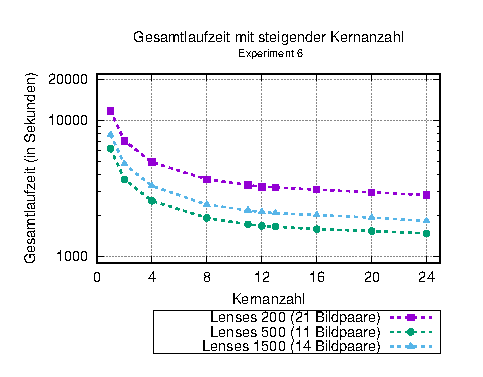
\includegraphics[width=\linewidth]{pdf/times_exp6}
				\caption{Experiment 6}
			\end{subfigure}
			\hfill
			\begin{subfigure}[b]{0.49\linewidth}
				\centering
				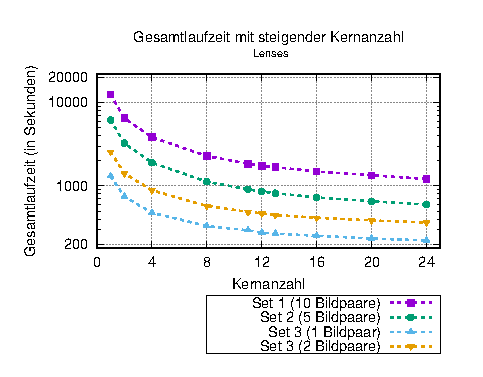
\includegraphics[width=\linewidth]{pdf/times_lenses}
				\caption{Lenses}
			\end{subfigure}
			\caption{Gesamtlaufzeiten}
		\end{figure}
	\end{center}
\end{frame}

\subsection{Profiling}
\begin{frame}[allowframebreaks]{Profiling}
	\begin{center}
		\begin{figure}[h]
			\hspace{-0.7cm}
			\begin{subfigure}[b]{0.4\linewidth}
				\centering
				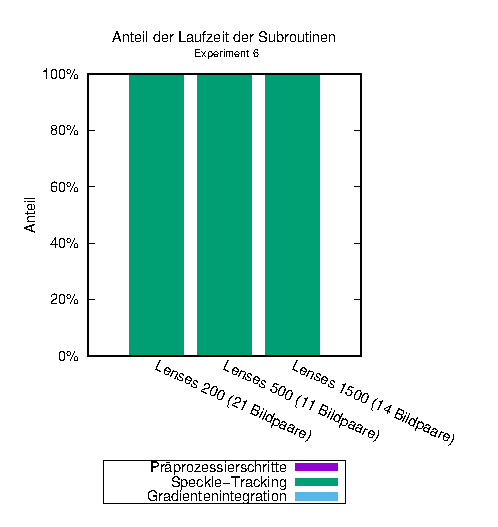
\includegraphics[width=\linewidth]{pdf/main_exp6.eps}
				\caption{Experiment 6}
			\end{subfigure}
			\hspace{-1.0cm}
			\begin{subfigure}[b]{0.4\linewidth}
				\centering
				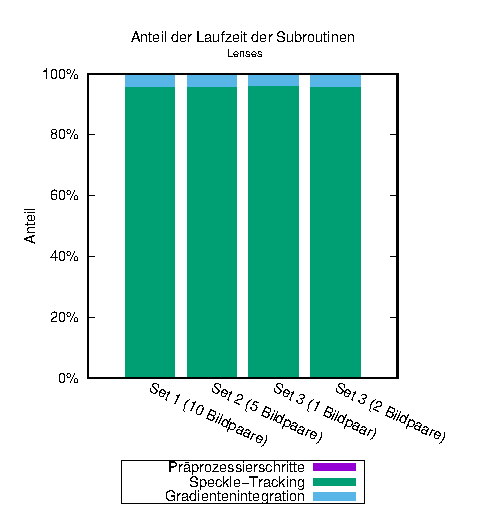
\includegraphics[width=\linewidth]{pdf/main_lenses.eps}
				\caption{Lenses}
			\end{subfigure}
			\hspace{-0.3cm}
			\begin{subfigure}[b]{0.33\linewidth}
				\centering
				\includegraphics[width=\linewidth]{pdf/graph_main_profiling}
				\caption{Algorithmus}
			\end{subfigure}
		\caption{Laufzeitanteile der Subroutinen}
		\end{figure}
		
		\framebreak
		\begin{figure}[h]
			\hspace{-0.6cm}
			\begin{subfigure}[b]{0.45\linewidth}
				\centering
				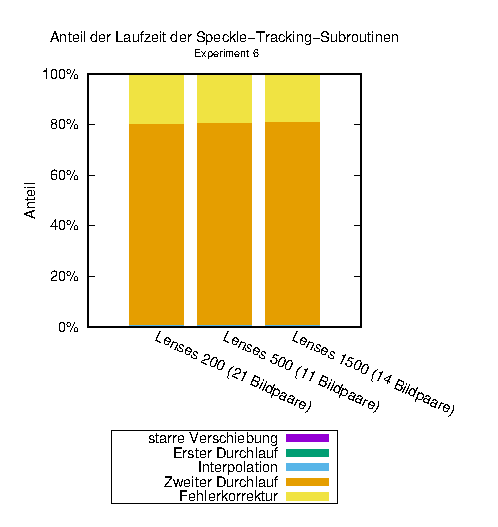
\includegraphics[width=\linewidth]{pdf/speckle_exp6.eps}
				\caption{Experiment 6}
			\end{subfigure}
			\hspace{-0.9cm}
			\begin{subfigure}[b]{0.45\linewidth}
				\centering
				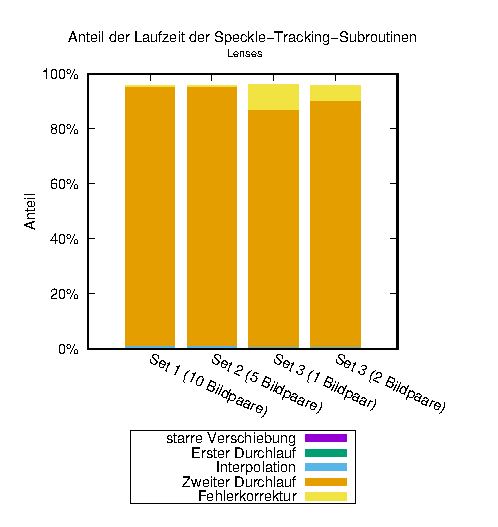
\includegraphics[width=\linewidth]{pdf/speckle_lenses.eps}
				\caption{Lenses}
			\end{subfigure}
			\hspace{-0.3cm}
			\begin{subfigure}[b]{0.19\linewidth}
				\centering
				\includegraphics[width=0.65\linewidth]{pdf/graph_speckle_profiling}
				\caption{Algorithmus}
			\end{subfigure}
			\caption{Laufzeitanteile der Speckle-Tracking-Routinen}
		\end{figure}
		
		\framebreak
		
		\begin{figure}[h]
			\begin{subfigure}[b]{0.45\linewidth}
				\centering
				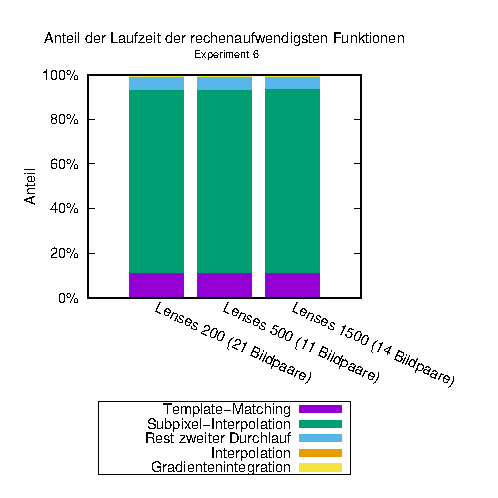
\includegraphics[width=\linewidth]{pdf/slow_exp6.eps}
				\caption{Experiment 6}
			\end{subfigure}
			\begin{subfigure}[b]{0.45\linewidth}
				\centering
				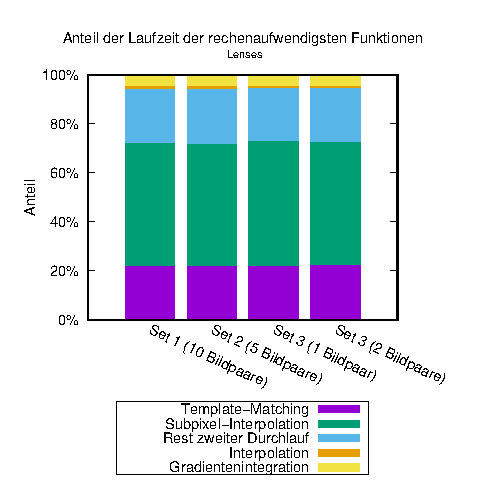
\includegraphics[width=\linewidth]{pdf/slow_lenses.eps}
				\caption{Lenses}
			\end{subfigure}
			\caption{Laufzeitanteile der rechenaufwendigsten Funktionen}
		\end{figure}
		\vspace{-0.35cm}
		\textbf{$ \Rightarrow $ über 95\%}
	\end{center}
\end{frame}
